% Standalone RAKL episode-to-governed-method loop (Paper III, Figure 1).
% Build:  pdflatex method_loop.tex  -> method_loop.pdf
\documentclass[border=6pt]{standalone}
\usepackage{tikz}
\usepackage{helvet}\renewcommand{\familydefault}{\sfdefault}
\usetikzlibrary{positioning,arrows.meta,shapes.geometric,fit,backgrounds,calc}
\definecolor{oiblue}{HTML}{0072B2}
\definecolor{oivermillion}{HTML}{D55E00}
\begin{document}
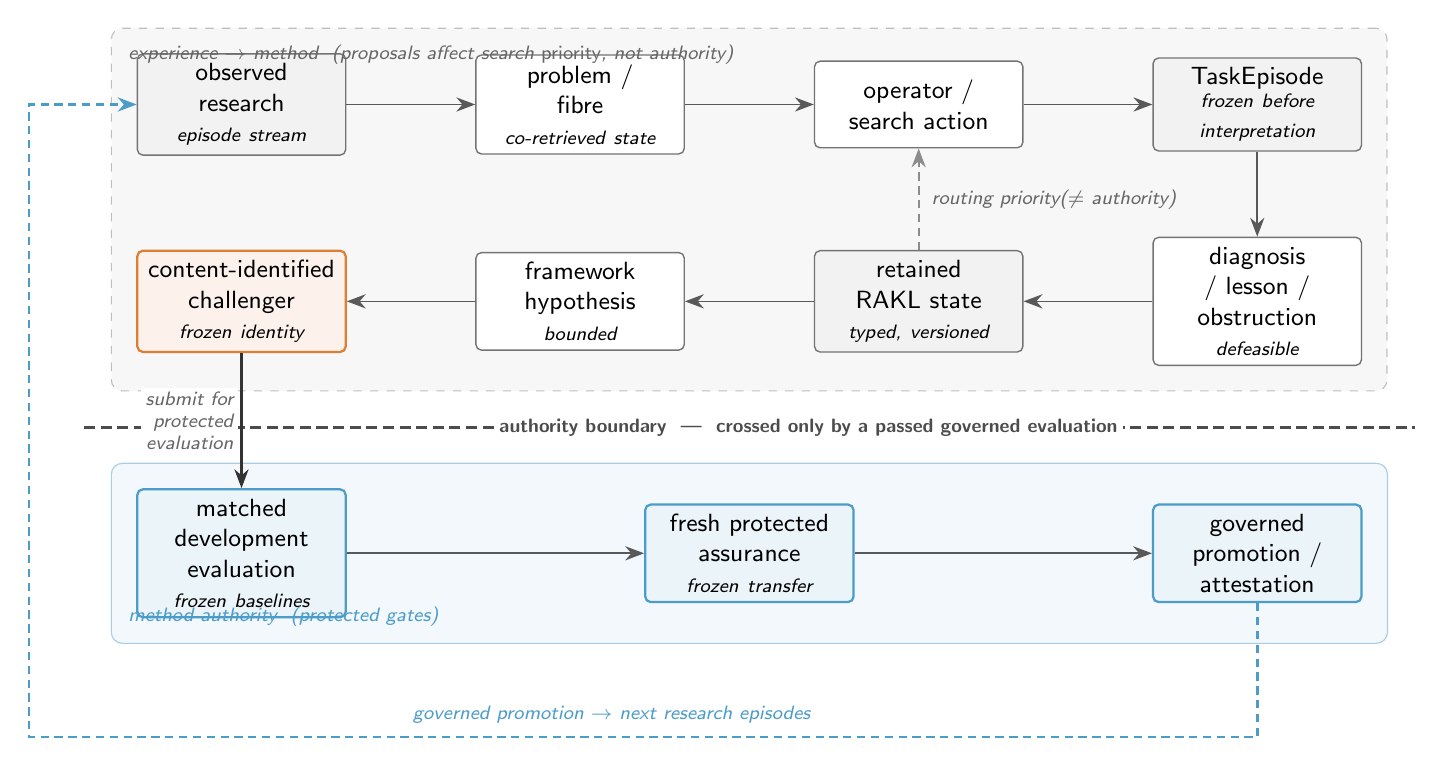
\begin{tikzpicture}[
  font=\small,
  >={Stealth[length=2.4mm]},
  bx/.style={rounded corners=2pt, draw=black!55, line width=0.5pt, align=center,
             inner sep=3.5pt, minimum height=11mm, text width=24mm, fill=white},
  store/.style={bx, fill=black!5},
  challenger/.style={bx, draw=oivermillion!80, line width=0.8pt, fill=oivermillion!8},
  authority/.style={bx, draw=oiblue!70, line width=0.8pt, fill=oiblue!8},
  flow/.style={->, line width=0.6pt, draw=black!65},
  softflow/.style={->, line width=0.6pt, draw=black!45, dash pattern=on 3pt off 2pt},
  cross/.style={->, line width=0.9pt, draw=black!80},
  lbl/.style={font=\scriptsize\itshape, text=black!60},
  sub/.style={font=\scriptsize\itshape},
]
% ---- Row 1 : observed research -> episode (left to right) ----
\node[store]      (obs) at (0,0)     {observed\\research\\{\itshape\scriptsize episode stream}};
\node[bx]         (fib) at (4.3,0)   {problem /\\fibre\\{\itshape\scriptsize co-retrieved state}};
\node[bx]         (op)  at (8.6,0)   {operator /\\search action};
\node[store]      (ep)  at (12.9,0)  {TaskEpisode\\{\itshape\scriptsize frozen before\\interpretation}};
% ---- Row 2 : diagnosis -> retained state -> hypothesis -> challenger (right to left) ----
\node[bx]         (diag) at (12.9,-2.5) {diagnosis / lesson /\\obstruction\\{\itshape\scriptsize defeasible}};
\node[store]      (state) at (8.6,-2.5) {retained\\RAKL state\\{\itshape\scriptsize typed, versioned}};
\node[bx]         (hyp)  at (4.3,-2.5)  {framework\\hypothesis\\{\itshape\scriptsize bounded}};
\node[challenger] (chal) at (0,-2.5)    {content-identified\\challenger\\{\itshape\scriptsize frozen identity}};
% ---- Authority row : matched eval -> fresh assurance -> governed promotion ----
\node[authority]  (mev) at (0,-5.7)    {matched development\\evaluation\\{\itshape\scriptsize frozen baselines}};
\node[authority]  (fresh) at (6.45,-5.7) {fresh protected\\assurance\\{\itshape\scriptsize frozen transfer}};
\node[authority]  (prom) at (12.9,-5.7)  {governed\\promotion /\\attestation};

% ---- Background bands ----
\begin{scope}[on background layer]
  \node[draw=black!25, dashed, rounded corners=4pt, fill=black!3,
        fit=(obs)(fib)(op)(ep)(diag)(state)(hyp)(chal), inner sep=9pt] (propband) {};
  \node[draw=oiblue!35, rounded corners=4pt, fill=oiblue!5,
        fit=(mev)(fresh)(prom), inner sep=9pt] (authband) {};
\end{scope}
\node[lbl, anchor=north west] at ($(propband.north west)+(1mm,-1mm)$)
      {experience $\rightarrow$ method\ \ (proposals affect search \emph{priority}, not authority)};
\node[lbl, anchor=south west, text=oiblue!70] at ($(authband.south west)+(1mm,1mm)$)
      {method authority\ \ (protected gates)};

% ---- Authority boundary (only a passed governed evaluation crosses) ----
\coordinate (bnL) at (-2.0,-4.1);
\coordinate (bnR) at (14.9,-4.1);
\draw[line width=1.3pt, black!70, dash pattern=on 4pt off 2pt] (bnL) -- (bnR);
\node[fill=white, inner sep=2pt, font=\scriptsize\bfseries, text=black!70, align=center]
      at (7.2,-4.1) {authority boundary\ \ ---\ \ crossed only by a passed governed evaluation};

% ---- Main flows ----
\draw[flow] (obs) -- (fib);
\draw[flow] (fib) -- (op);
\draw[flow] (op)  -- (ep);
\draw[flow] (ep)  -- (diag);
\draw[flow] (diag) -- (state);
\draw[flow] (state) -- (hyp);
\draw[flow] (hyp) -- (chal);
% challenger crosses the boundary downward into protected evaluation
\draw[cross] (chal.south) -- node[lbl, left, align=right, xshift=-1pt, fill=white, inner sep=1.5pt]{submit for\\protected\\evaluation} (mev.north);
\draw[flow] (mev) -- (fresh);
\draw[flow] (fresh) -- (prom);

% ---- Soft feedback : retained experience re-ranks routing, not authority ----
\draw[softflow] (state.north) -- node[lbl, right, xshift=1pt]{routing priority\\($\neq$ authority)} (op.south);

% ---- Governed promotion returns to next research episodes ----
\draw[->, line width=0.9pt, draw=oiblue!70, densely dashed]
     (prom.south) -- ++(0,-1.7) -| (-2.7,0) -- (obs.west);
\node[lbl, text=oiblue!70] at (4.7,-7.75)
      {governed promotion $\rightarrow$ next research episodes};
\end{tikzpicture}
\end{document}
